\documentclass[12pt,a4paper]{article}
\usepackage[utf8]{inputenc}
\usepackage[T1]{fontenc}
\usepackage[spanish,es-noquoting]{babel}
\usepackage{amsmath,amssymb}
\usepackage{booktabs}
\usepackage{lmodern}
\usepackage{graphicx}
\usepackage{siunitx}
\usepackage{geometry}
\usepackage{hyperref}

\geometry{margin=2.5cm}
\hypersetup{colorlinks=true, linkcolor=black, urlcolor=blue, citecolor=black}
\sisetup{output-decimal-marker={,}}

\title{Práctica 3 de Medioambiente: análisis del nivel de ruido ambiental}
\author{ }
\date{ }

\begin{document}

\maketitle

\section*{Resumen}
En esta práctica se analiza una serie temporal de niveles sonoros medidos en decibelios ponderados A, con el objetivo de caracterizar el ruido ambiental mediante el nivel continuo equivalente $L_{Aeq}$. A partir de 180 muestras se obtiene un valor medio equivalente de \SI{58.6029}{dBA} con una incertidumbre propagada de \SI{0.0093}{dB}, inferior al umbral de referencia de \SI{60}{dBA}. La diferencia respecto a la medida de aplicación utilizada en el script, \SI{59.4}{dBA}, también resulta negativa.

\section*{Objetivo}
El objetivo de la práctica es estudiar la evolución temporal del nivel de presión sonora medido y condensar la información de la serie en un único indicador energético, el nivel continuo equivalente. Este parámetro permite comparar una secuencia de medidas irregulares con límites normativos o valores de referencia establecidos para distintas áreas acústicas.

\section*{Fundamento teórico}
El nivel de presión sonora en escala logarítmica se define como
\[
L_A = 10\log_{10}\!\left(\frac{P^2}{P_0^2}\right),
\]
donde $P_0$ es la presión de referencia. Cuando se dispone de una serie de niveles medidos $L_i$, el nivel continuo equivalente se calcula como
\[
L_{Aeq} = 10\log_{10}\!\left(\frac{1}{N}\sum_{i=1}^{N}10^{L_i/10}\right),
\]
siendo $N$ el número de muestras.

Este promedio no se realiza directamente sobre los decibelios, sino sobre la magnitud lineal asociada a la energía acústica. Por ello, una pequeña variación en dB puede tener un efecto diferente cuando se transforma al dominio lineal.

\section*{Datos y procedimiento}
Se ha trabajado con una serie de $N=180$ medidas tomadas a intervalos regulares. El script asociado a la práctica utiliza los siguientes pasos:
\begin{enumerate}
    \item Construir el vector temporal de las medidas.
    \item Convertir cada valor de dB a magnitud lineal mediante $10^{L_i/10}$.
    \item Calcular el promedio energético y volver a la escala logarítmica.
    \item Comparar el resultado con un límite de referencia de \SI{60}{dBA} y con una medida de aplicación de \SI{59.4}{dBA}.
\end{enumerate}

Además, la serie presenta los siguientes estadísticos básicos:

\begin{table}[h]
\centering
\begin{tabular}{lc}
\toprule
{Magnitud} & {Valor} \\
\midrule
Número de muestras & 180 \\
Mínimo (dBA) & 53.2 \\
Máximo (dBA) & 65.8 \\
Media aritmética (dBA) & 57.8378 \\
Mediana (dBA) & 57.7 \\
Desviación típica (dBA) & 2.4028 \\
\bottomrule
\end{tabular}
\caption{Resumen descriptivo de la serie medida.}
\end{table}

\section*{Resultados}
El cálculo del nivel equivalente proporciona:
\[
L_{Aeq} = \left(58.6029 \pm 0.0093\right)\,\mathrm{dBA}.
\]
La incertidumbre propagada asociada al resultado es muy pequeña, del orden de $9.3\times 10^{-3}$ dB, debido a que las incertidumbres introducidas en las medidas individuales son muy reducidas.

La transformación lineal utilizada para el promedio energético permite además calcular los percentiles de la magnitud $10^{L/10}$ y expresarlos en escala logarítmica como niveles en dBA.

\begin{table}[h]
\centering
\begin{tabular}{cc}
\toprule
Percentil & Valor (dBA) \\
\midrule
90 & 60.8 \\
50 & 57.7 \\
10 & 55.1 \\
\bottomrule
\end{tabular}
\caption{Percentiles expresados en nivel sonoro (dBA).}
\end{table}

\begin{figure}[h]
\centering
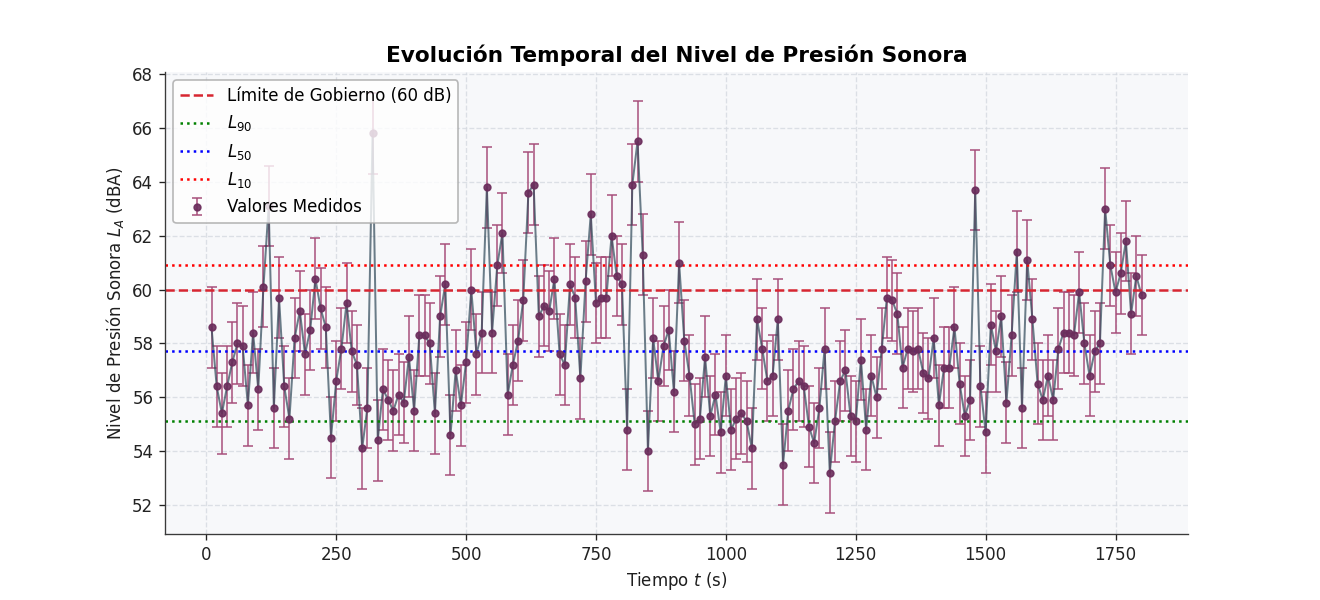
\includegraphics[width=0.95\linewidth]{plot_dba.png}
\caption{Evolución temporal del nivel de presión sonora en dBA.}
\end{figure}

La comparación con los valores de referencia es:
\[
L_{Aeq} - \SI{60}{dBA} = \SI{-1.3971}{dB},
\]
\[
L_{Aeq} - \SI{59.4}{dBA} = \left(-0.7971 \pm 0.0093\right)\,\mathrm{dB}.
\]
Por tanto, la media equivalente queda por debajo del límite de \SI{60}{dBA} y también por debajo de la medida de aplicación considerada en el análisis.

\subsection*{Interpretación}
La serie presenta oscilaciones moderadas y algunos picos aislados por encima de \SI{63}{dBA}, pero el comportamiento global se mantiene en torno a los \SI{58}{dBA}. El valor equivalente obtenido confirma que, en promedio energético, el nivel sonoro no supera el umbral de comparación fijado.

\section*{Conclusión}
La práctica permite comprobar cómo una serie temporal de ruido ambiental puede resumirse de forma robusta mediante el nivel continuo equivalente. En este caso, el entorno analizado muestra un comportamiento compatible con el valor de referencia de \SI{60}{dBA}. La diferencia negativa obtenida respecto al límite indica que la situación estudiada no lo sobrepasa en promedio.

\end{document}
